% v2_empirical_findings, generated from immutable frozen evidence; human author review pending.
\documentclass[conference]{IEEEtran}
\usepackage[T1]{fontenc}
\usepackage{amsmath,amssymb,booktabs,url}
\usepackage{tikz,pgfplots}
\pgfplotsset{compat=1.18}
\newcommand{\ind}{\mathbf{1}}
\title{Empirical Findings on Causal Temporal Matching:\\A Reproducible Visual Place Recognition Audit}
\author{\IEEEauthorblockN{Mingyang Zhou}\IEEEauthorblockA{University of Chinese Academy of Sciences\\\textit{Additional authors and correspondence pending}}}
\begin{document}\maketitle
\begin{abstract}
Sequential visual place recognition can improve image retrieval, but a gain over a single image does not establish the value of an adaptive decision rule. We audit a causal descriptor-score pipeline, fixed temporal and encoder-fusion controls, one predeclared confidence heuristic, and an adaptation of sequence-matching receptiveness prediction. Encoder weights are frozen; only Nordland training and validation determine the method settings. All compared methods share ground truth and startup exclusions within each dataset. On 292 validation queries, single-frame CosPlace, the selected fixed trajectory, and the heuristic obtain 71.92\%, 99.66\%, and 82.88\% Recall@1. A timestamped code-and-protocol freeze precedes a new St Lucia evaluation using geographic labels. On 1456 common queries, the same methods obtain 97.66\%, 98.63\%, and 98.83\%; fixed score blending reaches 99.52\%. Ordered-history and prescribed ablation controls are retained together with negative results. Real-image batch-one timings include decoding, preprocessing, encoding, history and ranking. At the prescribed $10$ m tolerance, single-frame and selected temporal recall are 95.05\% and 74.45\%, exposing unstable geographic transfer. The tested adaptive contribution remains unsubstantiated. The study provides a bounded, reproducible account of baseline strength, protocol transfer and deployment cost.
\end{abstract}
\begin{IEEEkeywords}visual place recognition, causal sequence matching, reproducibility, baseline comparison, protocol transfer\end{IEEEkeywords}

\section{Introduction}
Visual place recognition (VPR) retrieves a previously observed place from an image, often under changes in appearance and viewpoint~\cite{tutorial}. An image encoder produces a compact descriptor; the nearest reference descriptor gives an image-level place hypothesis. Sequential observations offer extra information: an isolated high similarity may become less credible when earlier queries do not support a compatible reference trajectory. Conversely, a visually ambiguous current frame may be resolved by consistent past observations.

This intuition does not justify every temporal or confidence mechanism. A simple fixed sequence can already solve most development errors, leaving little room for a further component. A heuristic can also suppress useful temporal evidence or restrict the candidate pool. Finally, a relative reference-index velocity selected on one video can transfer poorly to a dataset with different sampling and geographic ground truth. These issues matter when the empirical claim is an incremental method contribution rather than the usefulness of history in general.

We ask three bounded questions. How much does a causal fixed trajectory add beyond frozen single-frame and static-fusion controls? Does one train-statistic-based confidence rule add value over strong fixed choices and a related-code comparator? Which findings survive an independent protocol and genuine online computation? The method-selection budget is declared before development evaluation, the new test is opened only after an immutable freeze, and all unfavorable configurations remain available. We stop extending the heuristic after it fails the development superiority criterion.

The contribution is an empirical audit with matched query sets, exact prediction ledgers, causal tests, explicit source adaptations, and a documented negative adaptive hypothesis. Sequence matching, candidate reranking, confidence filtering and learned image descriptors are established ideas; we claim neither their invention nor a new network. The paper's numerical comparisons apply to the specified encoders, resolutions, galleries and ground-truth definitions.

\section{Related Work}
CosPlace~\cite{cosplace} and EigenPlaces~\cite{eigenplaces} provide learned global VPR descriptors; we use fixed checkpoints rather than retraining their encoders. DINOv2~\cite{dinov2} supplies a self-supervised representation as a contrasting frozen baseline. These configurations are compact instances of their model families and do not reproduce each paper's highest-performing benchmark setup.

SeqSLAM~\cite{seqslam} and the author-provided OpenSeqSLAM2.0 account~\cite{openseq} motivate reasoning over reference trajectories. Our implementation aggregates descriptor similarities causally; it does not reproduce the original grayscale difference and contrast-normalization pipeline. Delta Descriptors~\cite{delta} encode temporal changes; their centered formulation differs from the strictly past-and-current score window used here. Thus, descriptor trajectories are a baseline adaptation, not a claim to introduce sequence reasoning.

SMR~\cite{smr} predicts whether sequence matching helps using ratio features and a supervised receptiveness classifier. We execute fixed-source feature and training functions, while explicitly changing the encoder, training geography, labels and streaming evaluation. Its first-filter adaptation is reported separately from the original published benchmark. Image-matching reranking~\cite{match}, similarity-distribution uncertainty~\cite{doubt}, and reciprocal rank fusion (RRF)~\cite{rrf} provide additional context for candidate quality and confidence. The recent UPINLBS ResNet--Sinkhorn paper~\cite{sameconference} concerns global indoor VPR descriptors; its verified bibliographic record does not establish a complete mechanism-level novelty comparison. Its full text and the original SeqSLAM paper remained access-limited during this audit; the accessible author follow-up supports the sequence background.

\section{Pipeline and Predeclared Heuristic}
\subsection{Frozen Image-to-Ranking Pipeline}
Figure~\ref{fig:pipeline} separates online visual computation from offline labels. Each image is decoded to RGB, converted to a tensor, ImageNet-normalized and resized over the full frame to $224\times224$ with antialiasing. The frozen encoders output unit descriptors: CosPlace ResNet-18 and EigenPlaces ResNet-50 each have dimension $512$; DINOv2 ViT-S/14 uses a $384$-dimensional class token. These preprocessing choices are fixed across development and independent evaluation. No image encoder is trained in this study.

Let $x_t$ be the current unit query descriptor and $y_j$ an ordered gallery descriptor. We compute clipped cosine similarity $S_t(j)=x_t^\top y_j$ after float64 unit renormalization. Stable descending sorting retains gallery order for ties. The online matcher sees only score vectors and its internal history. Query filenames, ordinal labels, coordinates and positive sets are unavailable to its scoring API.

\begin{figure}[t]\centering
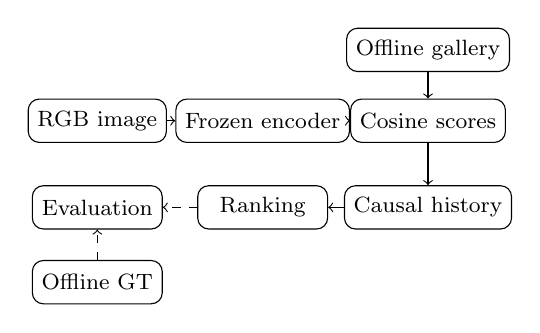
\begin{tikzpicture}[every node/.style={font=\footnotesize,align=center},box/.style={draw,rounded corners,minimum width=1.65cm,minimum height=.55cm}]
\node[box] (img) at (0,0) {RGB image};\node[box] (enc) at (2.1,0) {Frozen encoder};\node[box] (score) at (4.2,0) {Cosine scores};
\node[box] (gal) at (4.2,.9) {Offline gallery};\node[box] (hist) at (4.2,-1.1) {Causal history};\node[box] (rank) at (2.1,-1.1) {Ranking};\node[box] (eval) at (0,-1.1) {Evaluation};\node[box] (gt) at (0,-2.05) {Offline GT};
\draw[->] (img)--(enc);\draw[->] (enc)--(score);\draw[->] (gal)--(score);\draw[->] (score)--(hist);\draw[->] (hist)--(rank);\draw[->,dashed] (rank)--(eval);\draw[->,dashed] (gt)--(eval);
\end{tikzpicture}
\caption{The temporal pipeline uses current and past score rows. Labels enter only offline evaluation. Single-frame/static-fusion controls bypass temporal history. The output is a reference-image ranking, not a metric navigation estimate.}\label{fig:pipeline}
\end{figure}

\subsection{Fixed Causal Trajectory and Fusion Controls}
For a zero-based reference endpoint $j$, window $L$ and relative-index velocity set $V$, the temporal score is
\begin{equation}
T_t(j)=\max_{v\in V}\frac1L\sum_{\ell=0}^{L-1}S_{t-\ell}\!\left(j-\operatorname{rint}(v\ell)\right).
\label{eq:temporal}\end{equation}
Rounding follows ties-to-even. Any trajectory with an out-of-gallery index is invalid as a whole, with score $-\infty$. No future query is accessed. State resets at each traversal or split; the first $L-1$ queries use the single-frame ranking. For positive blend weights, invalid temporal paths stay invalid. At weight zero, the ranking is exactly single-frame. Known-range normalization $f(s)=(s+1)/2$ gives the fixed blend
\begin{equation}F_t(j)=(1-\lambda)f(S_t(j))+\lambda f(T_t(j)).\end{equation}

Development explores $L\in\{1,3,5,9\}$, $V\in\{\{.8\},\{1\},\{1.2\},\{.8,1,1.2\}\}$ and $\lambda\in\{0,.25,.5,.75,1\}$: the declared grid contains $80$ configurations, with single-frame/static and shuffled controls also retained. The validation-only deterministic selection chooses $L=9$, $V=\{1.2\}$, $\lambda=1$ for pure temporal matching and $\lambda=.75$ for the best interior blend at the same window and velocity. Reference-index velocity is not GPS speed. The independent window/velocity/reverse sensitivities are specified before test opening and never used to change those selections.

Static controls include EigenPlaces, DINOv2, fixed affine-normalized CosPlace--EigenPlaces mixtures and full-gallery RRF. RRF sums $1/(60+r)$ using one-based ranks from the two encoders. It needs no cross-model score calibration or trained coefficient. Static fusion always invokes both encoders; the temporal variants use CosPlace only.

\subsection{One Heuristic, without a Post-Test Search}
The heuristic reranks the current CosPlace Top-$50$ candidates and leaves its tail unchanged. It reuses the selected trajectory settings. Let $g_A$ and $g_T$ be the top-two finite-score gaps. Their training-only medians, fitted without labels on $592$ valid windows, are $m_A=0.02154516$ and $m_T=0.01837087$. Define ambiguity $a_t=\operatorname{clip}(1-g_A/m_A,0,1)$ and temporal support $b_t=\operatorname{clip}(g_T/m_T,0,1)$, with an epsilon floor $10^{-12}$.

The full temporal argmax endpoint is maintained as causal state. Continuity $c_t$ is the fraction of its last at most two increments within tolerance $1$ of the median velocity; the first valid endpoint uses $c_t=1$. Candidate agreement is $d_t=1$ when the endpoint belongs to the current Top-$50$, and $.25$ otherwise. The predeclared blend weight is
\begin{equation}\lambda_t=a_t b_t c_t d_t.\label{eq:adaptive}\end{equation}
This quantity is a heuristic weight, not a calibrated probability. If no candidate has a valid path, output reverts to the current ranking. We remove continuity, ambiguity and agreement separately, and replace the weight by fixed values on the identical candidate pool. No coefficients, new modules or window search are added after its failure on validation.

The score computation costs $O(NL|V|)$ with $O(NL)$ retained score storage for gallery size $N$. Our stable full-gallery sorting is $O(N\log N)$. The heuristic still computes the full trajectory before candidate reranking, so it does not reduce the encoding cost or establish an asymptotic search advantage. Dense gallery comparison and descriptor storage scale as $O(ND)$ for descriptor dimension $D$.

\subsection{SMR First-Filter Adaptation}
We pin the official SMR source commit and execute its unchanged selected functions under its MIT notice. Four ratio features use cosine-derived squared unit-descriptor distances, a length-nine unit-velocity diagonal, top rank one, epsilon $10^{-6}$ and group window two. Training uses the Nordland training queries only, with the original supervised four-class interpretation, StandardScaler, SMOTE and three hidden layers of $128$ units. Source defaults use random states $42$ for SMOTE and $0$ for the MLP. The single-configuration, five-fold source procedure is retained; because oversampling precedes its internal cross-validation, that score is not independent evidence.

Our full reference gallery, compact CosPlace encoder, ordinal tolerance and train size differ from the original multi-descriptor benchmark. We implement its first filter at a fixed all-trusted operating point, count rejected queries as retrieval misses, omit restoration, and transfer the classifier without St Lucia retraining. Training callbacks only change diagnostic output format. Source convolution and streamed float32 temporal sums agree on development top-ten rankings within the declared numeric bound. These limitations prevent a full published-reproduction claim.

\section{Data, Freeze and Evaluation Protocol}
\subsection{Three Distinct Data Roles}
Nordland-Part-2020~\cite{nordland} supplies paired summer/winter frames. The gallery has $1,750$ reference images. Query training uses verified one-based ordinals $1$--$600$, and validation uses $701$--$1000$, with their separation retained. Eligible references differ by at most five ordinals. This is a frame-order benchmark convention, not geographic ground truth. The candidate audit found CosPlace Top-$50$ recall of $300/300$ on the full validation split; it motivates checking a bounded reranker but does not predict a usable method gain. All primary validation methods share the first-eight exclusion, giving $292$ queries; all-query startup results are recorded separately.

The earlier $650$-query Nordland holdout and $200$-query Gardens Point night results had already been seen. They are historical/post-hoc evidence, never a new blind test or a source of V2 choices. Their original code, negative gate experiments, frozen result files and five-page paper remain preserved. This paper's new independent comparison uses St Lucia.

We retrieve the official formatted test-only St Lucia subset through the source-pinned VPR dataset downloader, citing its original collection~\cite{stlucia} and benchmark curation~\cite{benchmark}. It contains $1,549$ reference images and $1,464$ queries in one reference and one query traversal. Source pano identifiers recover each traversal and increasing original-frame order; the timestamp field is empty. All images are decoded and hashed before the freeze. UTM zone $56$ south, latitude band J, is consistent. Independent PROJ reprojection of all $3,013$ latitude/longitude pairs differs from labels by at most $1.48305$ m, within the predeclared rounding check.

Documentation describes nominal five-metre selection, but measured adjacent-position medians are $11.42$ m in the reference and $11.96$ m in the query trajectory. Original-frame gaps are irregular. We preserve that discrepancy and do not resample the data to fit the trajectory model. This permits an ordered-index transfer experiment, not a claim of uniformly timed motion or fixed physical speed.

\subsection{Geographic Labels and Common Masks}
St Lucia positives are references within Euclidean UTM distance $25$ m, consistent with the checked encoder benchmark's default geographic threshold. Sensitivities at $10$ and $50$ m are specified before test access. Coordinates generate offline labels only; they never drive similarity, velocity, gating or path choice. Every query has at least one eligible reference under each specified radius. A closed-set exclusion ledger is retained even though it is empty here. The same first-eight exclusion gives $1,456$ primary queries for every method. Excluded startup queries still update history and have separate full-stream results.

We report image retrieval Recall@$1/5/10$, paired rescues and harms versus CosPlace, and descriptive contiguous blocks of $100$ queries. Correlated video frames do not provide independent trials, and seed variation or three timing repeats is not treated as a confidence interval. The geographic and ordinal protocols are reported separately; absolute percentages across them are not a common-task accuracy comparison.

\subsection{Pre-Test Freeze and Genuine Online Cost}
A timestamped immutable packet stores code/test snapshots, source commits, encoder preprocessing and weight hashes, gallery identities, training statistics, the trained SMR classifier, all parameters, masks, thresholds, plots and the timing plan. Its recorded independent-performance flag is false. The first performance-access receipt follows the freeze, and all frozen source hashes are verified at evaluation. All $24$ predeclared independent configurations and the radius sensitivities remain in the public numeric evidence; no test-selected configuration replaces the development choice.

Accuracy extraction and timed queries both use batch one. Latency reopens and decodes every image, prepares the tensor, runs each required encoder, transfers its descriptor to CPU, computes gallery similarities, updates history and sorts the result. Cached scores are used only outside the timed interval for identity checks. On the RTX 3060 Laptop GPU, with PyTorch $2.6.0$ and CUDA $12.4$, each method receives $20$ warm images followed by three complete traversals with CUDA synchronization. CPU and BLAS threads are fixed to one, startup remains included and clocks are not locked. Dual-encoder methods prepare each encoder's input separately in this implementation; shared preprocessing could reduce their cost. Gallery extraction is an offline batch-sixteen operation; initialization and serialization are excluded from its per-encoder extraction timer and remain in the total command wall time.

\section{Results and Analysis}
\subsection{Fixed Controls and Transfer}
Table~\ref{tab:accuracy} compares the preselected methods using the same per-dataset query mask. On validation, pure fixed temporal retrieves $291/292$ correctly compared with $210/292$ for CosPlace. Its $82$ rescues and one harm show a large development gain; they do not prove an incremental adaptive contribution. The causal heuristic retrieves only $242/292$, and even its strongest prescribed component removal remains below mature fixed controls.

On independent St Lucia, the development-selected pure trajectory gains $14$ correct queries net over CosPlace, with $34$ rescues and $20$ harms. The fixed interior blend has $34$ rescues and $7$ harms. The heuristic has $17$ rescues and no harms; its apparent advantage over pure temporal disappears against stronger fixed blending and fixed candidate-pool controls. The transferred SMR adaptation also exceeds the heuristic under the primary radius. The primary result has an automated Outcome B label. The prescribed tighter tolerance reverses the selected temporal gain, requiring an overall Outcome C assessment of unstable transfer. The tested new rule has no established superiority over mature controls.

\begin{table*}[t]\centering\small
\caption{Recall percentages under distinct protocols. Nordland uses $292$ validation queries and ordinal tolerance $\pm5$; St Lucia uses $1,456$ independent queries and radius $25$ m. Rescue/harm is paired against CosPlace on St Lucia. Fixed T and blend are selected on validation. SMR* is the disclosed code adaptation.}\label{tab:accuracy}
\begin{tabular}{lrrrrrr}\toprule
Method & Nordland R@1 & St Lucia R@1 & St Lucia R@5 & St Lucia R@10 & Rescue & Harm\\\midrule
CosPlace A & 71.92 & 97.66 & 99.52 & 99.73 & 0 & 0\\
EigenPlaces B & 84.59 & 99.04 & 99.73 & 100.00 & 27 & 7\\
DINOv2 & 52.05 & 37.84 & 59.34 & 69.16 & 7 & 878\\
RRF & 83.22 & 98.97 & 99.86 & 100.00 & 19 & 0\\
Fixed A+B ($w_B=.75$) & 85.62 & 99.38 & 99.93 & 100.00 & 26 & 1\\
Fixed T ($L9,v1.2$) & 99.66 & 98.63 & 99.93 & 100.00 & 34 & 20\\
Fixed blend ($\lambda=.75$) & 98.97 & 99.52 & 100.00 & 100.00 & 34 & 7\\
Heuristic & 82.88 & 98.83 & 99.79 & 99.93 & 17 & 0\\
SMR* & 94.18 & 99.66 & 100.00 & 100.00 & 34 & 5\\
\bottomrule\end{tabular}\end{table*}

\subsection{Ablations and Sequence Controls}
Table~\ref{tab:ablations} separates the heuristic from weight replacement and component removal. Removing ambiguity helps the heuristic on validation, supporting the concern that a gap-based confidence veto can suppress useful evidence. This descriptive observation does not authorize another post-test rule. Fixed weights on the same Top-$50$ pool also exceed the full heuristic. Candidate coverage is therefore an upper bound, not evidence that the chosen weight extracts its available signal.

\begin{table}[t]\centering\small
\caption{Prescribed heuristic ablations and identical-pool fixed weights; R@1 percentages. No ablation is adopted using the independent result.}\label{tab:ablations}
\begin{tabular}{lrr}\toprule
Top-50 rule & Nordland & St Lucia\\\midrule
Full heuristic & 82.88 & 98.83\\
Without $c_t$ & 84.93 & 98.90\\
Without $a_t$ & 89.38 & 99.45\\
Without $d_t$ & 83.56 & 98.97\\
Fixed $\lambda=1$ & 98.29 & 99.18\\
Fixed $\lambda=.5$ & 94.86 & 99.73\\
Fixed $\lambda=.75$ & 97.95 & 99.59\\
\bottomrule\end{tabular}\end{table}

Figure~\ref{fig:sequence} retains the broad-velocity window sensitivity and shuffled-history control. Ordered histories exceed shuffled histories under each dataset's primary protocol; this control does not negate the selected trajectory's tighter-radius failure. The externally perfect length-five broad-velocity row is a predeclared sensitivity observation, not a newly selected final method. Reverse velocity is also unfavorable. Relative motion and sampling assumptions matter; selecting the best external window or velocity would change this test's role from independent validation to exploration.

\begin{figure}[t]\centering
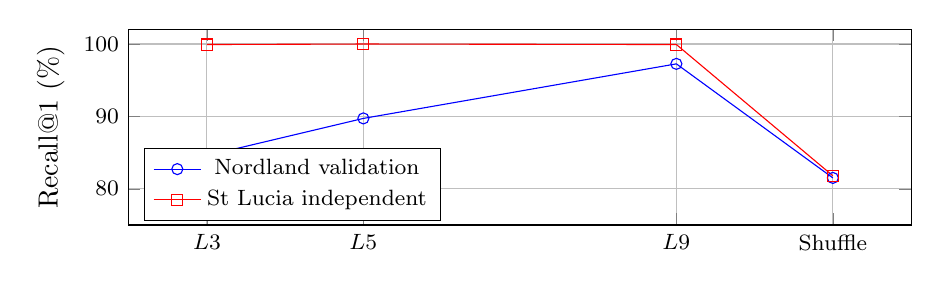
\begin{tikzpicture}\begin{axis}[width=.95\columnwidth,height=1.6in,ymin=75,ymax=102,xmin=2,xmax=12,xtick={3,5,9,11},xticklabels={$L3$,$L5$,$L9$,Shuffle},ylabel={Recall@1 (\%)},grid=major,legend style={font=\footnotesize,at={(.02,.02)},anchor=south west},tick label style={font=\footnotesize}]
\addplot+[mark=o] coordinates {(3,84.589041) (5,89.726027) (9,97.260274) (11,81.506849)};\addlegendentry{Nordland validation}
\addplot+[mark=square] coordinates {(3,99.931319) (5,100.000000) (9,99.931319) (11,81.799451)};\addlegendentry{St Lucia independent}
\end{axis}\end{tikzpicture}
\caption{Fixed $V=\{.8,1,1.2\}$, $\lambda=1$ with length sensitivity; Shuffle retains $L9$ and current query while permuting past history. Different GT/denominators across datasets; compare ordered and shuffled points within each role. These are prescribed controls, not test-driven parameter choices.}\label{fig:sequence}
\end{figure}

The source-pinned classifier has only three harmful-sequence and six both-wrong training examples before resampling; its source resampling and internal cross-validation cannot substitute for held-out transfer. Its protocol and model capacity also differ from the label-free heuristic. We therefore interpret this comparator as a related-code stress test and keep its adaptations and rejection counts visible. A method claim must survive both mature fixed controls and a genuinely comparable related method.

\subsection{Predeclared Geographic Tolerance Sensitivity}
Table~\ref{tab:radius} keeps the same $1,456$ queries at all prescribed radii. At $10$ m, single-frame recall is 95.05\%, whereas the selected pure trajectory obtains 74.45\%. The selected trajectory's net correct count changes from $-300$ at $10$ m to $+14$ at the primary $25$ m and $+30$ at $50$ m. The primary result is preserved, but it cannot support a uniformly improved geographic retrieval claim. A broad-neighborhood label can accept a temporal endpoint that a tighter tolerance rejects. Index-velocity mismatch and averaging are plausible contributors; this experiment does not establish a separate causal explanation or pose-error estimate. No tolerance or method is selected to conceal the reversal.
\begin{table}[t]\centering\small
\caption{Prescribed geographic radii, common $1,456$ queries; R@1 percentages. The primary radius remains $25$ m.}\label{tab:radius}
\begin{tabular}{lrrr}\toprule Method & $10$ m & $25$ m & $50$ m\\\midrule
CosPlace A & 95.05 & 97.66 & 97.94\\
Fixed T ($L9,v1.2$) & 74.45 & 98.63 & 100.00\\
Fixed blend ($\lambda=.75$) & 89.01 & 99.52 & 100.00\\
Heuristic & 95.40 & 98.83 & 98.90\\
SMR* & 86.06 & 99.66 & 100.00\\
\bottomrule\end{tabular}\end{table}

\subsection{Measured Batch-One Pipeline Cost}
Table~\ref{tab:latency} reports actual end-to-end latency. CosPlace's mean is 10.88 ms, of which preprocessing averages 5.63 ms and encoding plus CPU transfer 2.93 ms. Current-image decoding and preprocessing are consequently substantial; an encoder-only or cached-score timer would conceal practical cost. The temporal methods avoid a second visual encoder but still incur history and ranking work. SMR's measured pipeline includes its source ratio-feature computation and classifier, so it is not comparable to a published predictor-only timing.

\begin{table}[t]\centering\small
\caption{Real-image online latency in milliseconds: $20$ warm images, three full traversals ($4,392$ timed queries per method), batch one, synchronized CUDA. Startup included; clocks not locked. Small differences are descriptive.}\label{tab:latency}
\begin{tabular}{lrrr}\toprule Method & Mean & Median & P95\\\midrule
CosPlace A & 10.88 & 10.83 & 11.14\\
EigenPlaces B & 14.00 & 14.00 & 14.27\\
DINOv2 & 14.28 & 14.27 & 14.69\\
RRF & 23.17 & 23.18 & 23.47\\
Fixed A+B ($w_B=.75$) & 22.95 & 22.98 & 23.34\\
Fixed T ($L9,v1.2$) & 11.41 & 11.42 & 11.68\\
Fixed blend ($\lambda=.75$) & 11.30 & 11.31 & 11.55\\
Heuristic & 11.67 & 11.67 & 11.95\\
SMR* & 73.87 & 74.19 & 75.31\\
\bottomrule\end{tabular}\end{table}

Offline per-encoder gallery extraction takes 12.35, 15.21 and 16.89 s for CosPlace, EigenPlaces and DINOv2 respectively. Float32 gallery payloads and actual CPU/GPU residency are reported separately in the evidence; score histories are small for these galleries. CPU RSS includes audit arrays and allocator state, while CUDA allocated/reserved values do not represent total device memory. Neither these small-gallery costs nor warm-file-cache timings establish performance for a city-scale deployment.

\section{Discussion and Conclusion}
The development result demonstrates the danger of attributing a temporal gain to an extra component. The selected fixed trajectory is already near the validation ceiling. The heuristic's ambiguity, agreement and continuity factors can suppress history, and an apparent low-harm operating point is insufficient when fixed controls yield higher recall. On the independent protocol, the ordering among predeclared fixed variants also changes. This supports reporting window and motion sensitivity while preserving the original selection and unfavorable evidence. The tighter-radius reversal also cautions against treating a correct broad-neighborhood endpoint as precise localization.

Several validity limits remain. Nordland uses ordinal rather than geographic labels, and historical exact-frame repetitions and uncertain correspondence can distort its seen holdout. St Lucia is one curated route pair, with irregular spacing, loop revisits and positional-label uncertainty. Its measured spacing differs from documentation. Upstream encoder pretraining overlap is not audited; independence here concerns our method development. Compact checkpoints, full-frame resizing, dense search, candidate truncation, source SMR adaptations, uncalibrated heuristic weights, serial correlation and unlocked clocks bound interpretation. Retrieval recall does not establish localization RMSE, navigation success or robotic deployment. The access-limited same-conference paper also leaves a complete novelty comparison pending human review.

The paired ledgers support the following limited empirical conclusion: causal temporal ordering can improve broad-neighborhood retrieval here, its gains are unstable under tighter geographic tolerance, strong fixed choices are indispensable controls, and the tested adaptive contribution is not demonstrated. Future studies would need new development data and a new independent freeze before exploring a revised mechanism. The present evidence is preserved as a research audit rather than repaired by further test-based tuning.

\section*{Reproducibility and AI Disclosure}
Source versions, finite grids, source/licence receipts, train-statistic and model hashes, freeze/access timestamps, per-query and contiguous-block results, real latency samples, failures, and claim mappings are archived on the research branch of \url{https://github.com/zhoumy0313/upinlbs-2026-vpr}. Dataset photos and external pretrained checkpoints are retained locally with source URLs and hashes. This draft used OpenAI ChatGPT/Codex for code generation, test and analysis scripts, figure code, manuscript drafting and revision throughout the paper. Official encoder and SMR source attribution is preserved. Human authors must verify all code, scientific interpretation, citations, wording and authorship before submission; additional authors, correspondence, funding and conference-format details remain pending. No submission or author approval is implied.

\begin{thebibliography}{15}
\bibitem{tutorial} S. Schubert, P. Neubert, S. Garg, M. Milford, and T. Fischer, ``Visual place recognition: A tutorial,'' \emph{IEEE Robot. Autom. Mag.}, vol.31, no.3, pp.139--153, 2024, doi:10.1109/MRA.2023.3310859.
\bibitem{cosplace} G. Berton, C. Masone, and B. Caputo, ``Rethinking visual geo-localization for large-scale applications,'' in \emph{CVPR}, 2022, pp.4878--4888.
\bibitem{eigenplaces} G. Berton, G. Trivigno, B. Caputo, and C. Masone, ``EigenPlaces: Training viewpoint robust models for visual place recognition,'' in \emph{ICCV}, 2023, pp.11080--11090.
\bibitem{dinov2} M. Oquab \emph{et al.}, ``DINOv2: Learning robust visual features without supervision,'' arXiv:2304.07193, 2023.
\bibitem{seqslam} M. J. Milford and G. F. Wyeth, ``SeqSLAM: Visual route-based navigation for sunny summer days and stormy winter nights,'' in \emph{ICRA}, 2012, pp.1643--1649, doi:10.1109/ICRA.2012.6224623.
\bibitem{openseq} B. Talbot, S. Garg, and M. Milford, ``OpenSeqSLAM2.0: An open source toolbox for visual place recognition under changing conditions,'' arXiv:1804.02156v2, 2018.
\bibitem{delta} S. Garg, B. Harwood, G. Anand, and M. Milford, ``Delta descriptors: Change-based place representation for robust visual localization,'' \emph{IEEE Robot. Autom. Lett.}, vol.5, no.4, pp.5120--5127, 2020, doi:10.1109/LRA.2020.3005627.
\bibitem{smr} S. Hussaini, T. Fischer, and M. Milford, ``Improving visual place recognition with sequence-matching receptiveness prediction,'' in \emph{IROS}, 2025, pp.11073--11080, doi:10.1109/IROS60139.2025.11247581.
\bibitem{match} D. Sferrazza, G. Berton, G. Trivigno, and C. Masone, ``To match or not to match: Revisiting image matching for reliable visual place recognition,'' in \emph{CVPR Workshops}, 2025, pp.2874--2885.
\bibitem{doubt} E. Miller, M. Milford, M. B. Hafez, S. Ramchurn, and S. Ehsan, ``Through the lens of doubt: Robust and efficient uncertainty estimation for visual place recognition,'' \emph{IEEE Robot. Autom. Lett.}, vol.11, no.5, pp.5899--5906, 2026, doi:10.1109/LRA.2026.3674688.
\bibitem{rrf} G. V. Cormack, C. L. A. Clarke, and S. B\"uttcher, ``Reciprocal rank fusion outperforms condorcet and individual rank learning methods,'' in \emph{SIGIR}, 2009, pp.758--759, doi:10.1145/1571941.1572114.
\bibitem{sameconference} Y. Wei, Y. Li, and Z. Zheng, ``Balancing accuracy and efficiency: A ResNet--Sinkhorn framework for extracting global image descriptors in indoor visual place recognition,'' in \emph{UPINLBS}, 2025, pp.1--6, doi:10.1109/UPINLBS68186.2025.11468446.
\bibitem{stlucia} M. J. Milford and G. F. Wyeth, ``Mapping a suburb with a single camera using a biologically inspired SLAM system,'' \emph{IEEE Trans. Robot.}, vol.24, no.5, pp.1038--1053, 2008, doi:10.1109/TRO.2008.2004520.
\bibitem{benchmark} G. Berton, R. Mereu, G. Trivigno, C. Masone, G. Csurka, T. Sattler, and B. Caputo, ``Deep visual geo-localization benchmark,'' in \emph{CVPR}, 2022, pp.5396--5407.
\bibitem{nordland} S. Garg, ``Nordland-Part-2020,'' Zenodo, 2020, doi:10.5281/zenodo.4016653.

\end{thebibliography}
\end{document}
